
\section{Εισαγωγή}

%Ένα από τα βασικότερα προβλήματα στις σύγχρονες κοινωνίες είναι οι συλλογικές αποφάσεις. Χαρακτηριστικό παράδειγμα αποτελούν οι εκλογές στις οποίες όλοι οι πολίτες καλούνται να δηλώσουν τον υποψήφιο που προτιμούν με σκοπό την επιλογή του συνολικά καλύτερου υποψηφίου. Αυτού του είδους τα προβλήματα έχουν μελετηθεί από τη σκοπιά της κοινωνιολογίας κυρίως, όμως πρόσφατα έχει μελετηθεί και από τη σκοπιά της επιστήμης των υπολογιστών. ++


Στη παρούσα διπλωματική εργασία θα ασχοληθούμε με το πρόβλημα της χωροθέτησης υπηρεσιών. Υποθέτουμε ότι ένα σύνολο παικτών βρίσκονται σε ένα χώρο και εμείς επιθυμούμε να τοποθετήσουμε υπηρεσίες σε διαφορετικές θέσεις στο χώρο αυτό. Το κόστος κάθε παίκτη είναι η απόσταση του από τη πλησιέστερη υπηρεσία. Στόχος μας είναι να βρούμε τις βέλτιστες θέσεις ώστε το συνολικό κόστος των παικτών να είναι όσο το δυνατόν μικρότερο. Το συγκεκριμένο πρόβλημα έχει μελετηθεί εκτενώς τόσο στο πεδίο της επιστήμης των υπολογιστών όσο και στο πεδίο της επιχειρησιακής έρευνας. Ο λόγος είναι ότι μοντελοποιεί πληθώρα προβλημάτων, όπως τη επιλογή των θέσεων χτισίματος καινούριων βιβλιοθηκών από την κυβέρνηση βάση των προτιμήσεων των πολιτών. 

Αν γνωρίζουμε τις πραγματικές τοποθεσίες των παικτών τότε μπορούμε να προσεγγίσουμε τη βέλτιστη λύση αρκετά καλά. Ωστόσο, υπάρχουν πολλές εφαρμογές που οι θέσεις των παικτών δεν είναι δημοσίως γνωστές και πρέπει να δηλώνονται στην κεντρική αρχή από στρατηγικούς παίκτες. Κάθε παίκτης έχει στόχο να ελαχιστοποιήσει το κόστος του, χωρίς να τον εδιαφέρει το συνολικό κόστος. Τώρα ο στόχος δεν είναι μόνο να βρούμε τις θέσεις των υπηρεσιών αλλά να τις βάλουμε με τέτοιο τρόπο που κανένας παίκτης δεν μπορεί να κερδίσει δηλώνοντας ψευδή τοποθεσία. Ενδιαφερόμαστε λοιπόν για το σχεδιασμό φιλαληθών μηχανισμών για για προβλήματα χωροθέτισης.

Σε πολλά προβλήματα σχεδιασμού μηχανισμών, όπως οι δημοπρασίες, εισάγουμε στο μοντέλο πληρωμές για να εγγυηθούμε ότι η ανάθεση των αγαθών γίνεται με φιλαλήθη τρόπο. Όμως, σε περιβάλλον κοινωνικής επιλογής όπως τα προβλήματα χωροθέτησης υπηρεσιών, μπορεί να είναι παράνομο ή ανήθικο να επιβάλουμε πληρωμές. Πάνω σε αυτή την ιδέα ξεκίνησε η εύρενα από τους rocaccia και Tennenholtz \cite{Procaccia2013} πάνω στο σχεδιασμό προσεγγιστικών μηχανισμών χωρίς χρήματα. 

\section{Προβλήματα Χωροθέτησης}

Πρώτα θα ορίσουμε το βασικό μοντέλο του προβλήματος. Έχουμε ένα μετρικό χώρο $(X,d)$, όπου $d:X \times X  \rightarrow \mathbb{R}_{+}$ είναι μια συνάρτηση απόστασης μεταξύ των σημείων του χώρου. Η συνάρτηση είναι μετρική που σημαίνει ότι $\forall x,y,z \in Z$: $d(x,x)=0$ (ταύτιση), $d(x,y)=d(y,x)$ (συμμετρία) και $d(x,z)\le d(x,y)+d(y,z)$ (τριγωνική ανισότητα). Οι παίκτες έχουν μια ιδανική τοποθεσία στον χώρο. Ένα στιγμιότυπο αποτελείται από τις θέσεις των παικτών στο χώρο $\x=(x_1,...,x_n)$. 


Κάθε παίκτης δηλώνει τη θέση του στο μηχανισμό $M$. Ένας ντετερμινιστικός μηχανισμός είναι μία συνάρτηση που απεικονίζει το σύνολο των δηλωθέντων θέσεων των παικτών $\x$ σε $k$ υπηρεσίες $(c_1,...,c_k)$. Αντίστοιχα ένας τυχαιοποιημένος μηχανισμός $M$ απεικονίζει το σύνολο των δηλωθέντων θέσεων των παικτών $\x$ σε μια πιθανοτική κατανομή από $k$ υπηρεσίες. $(c_1,...,c_k)$.  


 Tο κόστος κάθε παίκτη είναι η απόσταση του από τη πλησιέστερη υπηρεσία, $cost(x_i,M(\x)) = min_{1\le j \le k} \{d(x_i,c_j) \}$. Το κοινωνικό κόστος ενός μηχανισμού $M$ είναι το άθροισμα των κοστών των παικτών, $ cost(\x,M(\x)) = \sum_{i=1}^{n} cost(x_i,\CC)$.
 
 Κάθε παίκτης είναι στρατηγικός και έχει στόχο να ελαχιστοποιήσει το κόστος του. Ο μηχανισμός έχει στόχο να ελαχιστοποιήσει το κοινωνικό κόστος. Η διαφορά αυτή ωθεί τους παίκτες να δηλώσουν ψευδή τοποθεσία για να κερδίσουν. Για αυτό ενδιαφερόμαστε για φιλαλήθης μηχανισμούς που σημαίνει ότι κανένας παίκτης δεν μπορεί να κερδίσει λέγοντας ψέματα.
 
 Στη συνέχεια θα δούμε τα βασικά αποτελέσματα για προβλήματα χωροθέτησης υπηρεσιών. Πρώτα θα αναλύσουμε τη περίπτωση που οι παίκτες είναι τοποθετημένοι στη γραμμή και στη συνέχεια τη περίπτωση που οι παίκτες είναι τοποθετημένοι σε δέντρα.
 
 
 
 
\subsection*{Μια υπηρεσία στη γραμμή}

Όταν θέλουμε να τοποθετήσουμε μια υπηρεσία, η θέση του διάμεσου παίκτη είναι βέλτιστη και ταυτόχρονα είναι φιλαλήθης. Η βασική ιδέα είναι ότι ο μοναδικός τρόπος που ένας παίκτης μπορεί να αλλάξει τη θέση της υπηρεσίας είναι να δηλώσει μια θέση από τη ``άλλη" μεριά του διάμεσου. Αυτό, όμως, θα έχει ως αποτέλεσμα η υπηρεσία να πάει πιο μακριά σε σχέση με τη πραγματική του θέση. Άρα δεν υπάρχει τρόπος κάποιος παίκτης να κερδίσει λέγοντας ψέματα.

\begin{theoremgr}[\cite{Moulin1980}]
Ο μηχανισμός που τοποθετεί την υπηρεσία στο διάμεσο παίκτη είναι βέλτιστος και φιλαλήθης.
 \end{theoremgr}

\begin{figure}[ht]
    \centering
    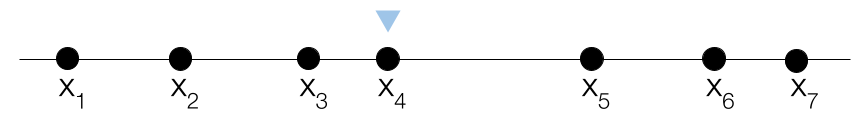
\includegraphics[width=0.6\textwidth]{Images/Median.png}
    \caption{Βέλτιστη λύση για μία υπηρεσία στη γραμμή}
    \label{fig:med}
\end{figure}

 
\subsection*{Δύο υπηρεσίες στη γραμμή}

Όταν θέλουμε να τοποθετήσουμε δύο υπηρεσίες το πρόβλημα γίνεται πιο δύσκολο. Αρχικά, μπορούμε εύκολα να δούμε ότι η βέλτιστη λύση δεν είναι φιλαλήθης. Μπορούμε να χωρίσουμε τους παίκτες σε δύο σύνολα, το δεξί και το αριστερό, ανάλογα με την υπηρεσία που προτιμούν. Όμως ένας παίκτης μπορεί να δηλώσει μια θέση που να τον βάζει στο άλλο σύνολο από αυτό που ανήκει πραγματικά, έτσι ώστε να φέρει την υπηρεσία του εκείνου του συνόλου πιο κοντά στην πραγματική του θέση. 


 
Ο μόνος τρόπος που μπορούμε να τοποθετήσουμε τις υπηρεσίες με φιλαλήθη τρόπο είναι να τις βάλουμε στο πιο δεξί και στον πιο αριστερό παίκτη. Παρατηρούμε ότι υποχρεωτικά ο πιο αριστερός παίκτης ανήκει στο αριστερό σύνολο και αντίστοιχα ο πιο δεξιά παίκτης ανήκει στο δεξί σύνολο. Με αυτό το τρόπο εξασφαλίζουμε φραγμένο λόγο προσέγγισης. Επιπλέον, τοποθετώντας τις υπηρεσίες στις ακριανές θέσεις παρατηρούμε ότι κανένας παίκτης δεν μπορεί να κερδίσει δηλώνοντας διαφορετική, αφού ο μόνος τρόπος να αλλάξει θέση μία υπηρεσία είναι να πάει πιο μακριά. 




\begin{figure}[ht]
    \begin{subfigure}[b]{\textwidth}
        \centering
        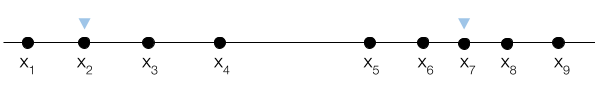
\includegraphics[width=0.8\textwidth]{Images/OPT2.png}
        \caption{Βέλτιστη ανάθεση}
        \label{fig:opt2}
     \end{subfigure}
    \hspace{20pt}
     \begin{subfigure}[b]{\textwidth}
        \centering
        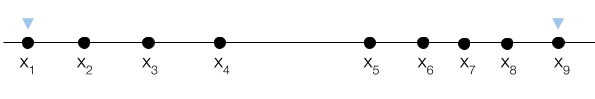
\includegraphics[width=0.8\textwidth]{Images/TwoExtremes.png}
        \caption{Ανάθεση στους δύο ακριανούς παίκτες}
        \label{fig:twoEx}
    \end{subfigure}
\end{figure}

\begin{theoremgr}[\textsc{Two Extremes  \cite{Procaccia2013}}]
Ο μηχανισμός που τοποθετεί τις υπηρεσίες στους δύο ακριανούς παίκτες είναι φιλαλήθης και έχει λόγο προσέγγισης $(n-2)$. 
\end{theoremgr}

Ο \textsc{Two Extremes} είναι ο μοναδικός ντετερμινιστικός μηχανισμός με φραγμένο λόγο προσέγγισης \cite{Fotakis2014}. Αν επιτρέψουμε στο μηχανισμό να χρησιμοποιήσει τυχαιότητα μπορούμε να πετύχουμε πολύ καλύτερο λόγο προσέγγισης. Ο proportional μηχανισμός είναι φιλαλήθης και έχει σταθερό λόγο προσέγγισης. Διαισθητικά τοποθετεί τη πρώτη υπηρεσία τυχαία σε μια από τις θέσεις των παικτών και τη δεύτερη τη τοποθετεί στη θέση κάποιου παίκτη με πιθανότητα ανάλογη της απόστασης του από τη πρώτη υπηρεσία.

\begin{definitiongr}[Propotional Μηχανισμός \cite{Lu2010}]
Για ένα στιγμιότυπο $\vec{x}=(x_1,...x_n)$, οι θέσεις των δύο υπηρεσιών επιλέγονται με τη παρακάτω τυχαία διαδικασία:
\begin{itemize}
    \item\textbf{Βήμα 1:} Επιλέγουμε ένα $i\in N$ τυχαία. Τοποθετούμε τη πρώτη υπηρεσία  $c_1$ στη θέση $x_i$

    \item\textbf{Βήμα 2:} Έστω $d_j = d(c_1,x_j)$ η απόσταση του παίκτη $j$ από τη πρώτη τοποθεσία. Επιλέγουμε το $j$ με πιθανότητα $\frac{d_j}{\sum_{k\in N}d_k}$. Τοποθετούμε τη δεύτερη υπηρεσία $c_2$ στη θέση $x_j$.
\end{itemize}
\end{definitiongr}

\begin{theoremgr} 
 O Proportional μηχανισμός είναι φιλαλήθης και έχει λόγο προσέγγισης το πολύ 4.
\end{theoremgr}

\subsection*{Περισσότερες από δύο υπηρεσίες στη γραμμή}

Όπως είδαμε το πρόβλημα γίνεται αρκετά πιο δύσκολο ακόμα και αν θέλουμε να τοποθετήσουμε μόνο δύο υπηρεσίες στη γραμμή. Δεν μπορούμε λοιπόν να περιμένουμε καλύτερα αποτελέσματα όταν θέλουμε να τοποθετήσουμε περισσότερες από δύο υπηρεσίες. Στη πραγματικότητα μπορούμε να δείξουμε ότι δεν υπάρχει ντετερμινιστικός φιλαλήθης μηχανισμός με φραγμένο λόγο προσέγγισης για $k\ge3$. Αυτό ισχύει ακόμα και για στιγμιότυπα με 4 παίκτες και 3 υπηρεσίες. Μπορούμε να δείξουμε ότι, όπως και πριν, οι δύο υπηρεσίες πρέπει να τοποθετηθούν στους δύο ακριανούς παίκτες για να είναι φιλαλήθης ο μηχανισμός. Η βασική ιδέα της απόδειξης είναι ότι δεν μπορούμε με φιλαλήθη τρόπο να επιλέξουμε σε ποιο παίκτη θα τοποθετηθεί η υπηρεσία. 

\begin{theoremgr}[\cite{Fotakis2014}]
Δεν υπάρχει ντερμινιστικός φιλαλήθης μηχανισμός με φραγμένο λόγο προσέγγισης για $k\ge3$.
\end{theoremgr}

Υπάρχει μια πολύ σημαντική οικογένεια ντετερμινιστικών μηχανισμών για προβλήματα χωροθέτησης. Διαισθητικά η οικογένεια των percentile μηχανισμών ``σπάει" το στιγμιότυπο σε τμήματα σύμφωνα με ένα διάνυσμα $\vec{p}$ και τοποθετεί μία υπηρεσία σε κάθε τμήμα. 

\begin{definitiongr}[$\vec{p}$-Percetntile Μηχανισμός \cite{Sui2013}]
    Ένας percentile μηχανισμός έχει ένα προκαθορισμένο διάνυσμα $\vec{p}=(p_1,...,p_k)$ τέτοιο ώστε $0\le p_1\le...\le p_k \le 1$. Ο μηχανισμός τοποθετεί τη $j$-οστή υπηρεσία στο $p_j$-οστό τμήμα του στιγμιότυπου. 
\[ c_j = x_{i_j}\; :\; i_j = \lfloor (n-1)\cdot p_j \rfloor +1 \]
\end{definitiongr}

Παράδειγμα του $(0.25,0.75)$-percentile μηχανισμού. Σε ένα στιγμιότυπο με 9 παίκτες ο μηχανισμός θα τοποθετεί τις υπηρεσίες στον 3ο παίκτη ($\lfloor 8\cdot 0.25 \rfloor +1  = 3$) και στον 7ο παίκτη ($\lfloor 8\cdot 0.75 \rfloor +1 = 7$), ανεξάρτητα από τις θέσεις των παικτών.
    \begin{center}
        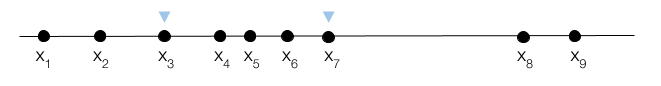
\includegraphics[width=0.8\textwidth]{Images/percentile.png}
    \end{center}

Αυτοί οι μηχανισμοί είναι φιλαλήθης για κάθε $k\ge2$. Είναι πολύ σημαντικό να σημειώσουμε ότι το διάνυσμα είναι προκαθορισμένο και δεν εξαρτάται από το στιγμιότυπο. Αυτός είναι και ο λόγος που είναι φιλαλήθης οι μηχανισμοί. Οι υπηρεσίες τοποθετούνται σε συγκεκριμένες θέσεις στο στιγμιότυπο ανεξάρτητα από τις θέσεις των παικτών. Ο μόνος τρόπος κάποιος παίκτης να αλλάξει τη θέση μια υπηρεσίας είναι να δηλώσει τοποθεσία σε άλλο τμήμα. Όπως στη μία υπηρεσία και το διάμεσο παίκτη, αυτή η αλλαγή θα πάει την υπηρεσία πιο μακριά. Το μειονέκτημα αυτών των μηχανισμών είναι ότι δεν έχουν πεπερασμένο λόγο προσέγγισης για $k\ge3$, όπως μας υποδηλώνει και το προηγούμενο θεώρημα. Ο μόνος percentile μηχανισμός με φραγμένο λόγο προσέγγισης είναι ο $(0,1)$-percentile μηχανισμός που είναι ισοδύναμος με τον \textsc{Two Extremes} μηχανισμό. Σε κάθε άλλη περίπτωση μπορούμε να δημιουργήσουμε ένα στιγμιότυπο στο οποίο οι παίκτες που έχουν υπηρεσίες στις θέσεις τους να είναι κοντά μεταξύ τους ενώ οι παίκτες που δεν έχουν υπηρεσίες να είναι μακριά. Αφού οι μηχανισμοί δεν ``κοιτούν" το στιγμιότυπο θα έχουν πολύ κακό λόγο προσέγγισης.

Είναι πολύ σημαντικό να παρατηρήσουμε ότι ο μόνος τρόπος για να έχουμε φραγμένο λόγο προσέγγισης είναι να τοποθετήσουμε μια υπηρεσία σε κάθε βέλτιστο cluster, δηλαδή σε κάθε ομάδα που εξυπηρετείται από την ίδια υπηρεσία στη βέλτιστη λύση. Όμως αυτό δεν μπορούμε να το πετύχουμε με φιλαλήθη τρόπο διότι η δομή των ομάδων αλλάζει όταν ένας παίκτης δηλώνει ψευδή τοποθεσία. Αυτό το εκμεταλλεύονται οι παίκτες για να κερδίσουν. Αν, από την άλλη, θέλουμε να έχουμε φιλαλήθης μηχανισμούς δεν πρέπει να ``κοιτάμε" τη δομή των ομάδων χάνοντας όμως το πεπερασμένο λόγο προσέγγισης. 

Από την άλλη πλευρά, μπορούμε να πετύχουμε καλύτερα αποτελέσματα αν επιτρέψουμε στους μηχανισμούς να χρησιμοποιήσουν τυχαιότητα. Πρώτα προτάθηκε ο  \textsc{Inversely Proportional Μηχανισμός} \cite{escoffier2011}, ο οποίος είναι $n/2$-προσεγγιστικός για $k$-υπηρεσίες με $n=k+1$ παίκτες. Έπειτα, προτάθηκε ο \textsc{Equal Cost} \cite{Fotakis2013sp} για $k$ υπηρεσίες και αυθαίρετο αριθμό παικτών, ο οποίος πετυχαίνει λόγο προσέγγισης το πολύ $n$. 


\begin{table}[ht]
    \centering
    \begin{tabular}{|c|c|c|c|}
         \hline
         & $k=1$ & $k=2$ & $k\ge3$ \\ \hline 
        Ντερμινιστικός & 1\cite{Moulin1980} & $n-2$ \cite{Procaccia2013} & $\infty$ \cite{Fotakis2013}\\ \hline
        Τυχαιοποιημένος & 1\cite{Moulin1980} & 4 \cite{Lu2010} & $n$ \cite{Fotakis2013sp} \\ \hline
    \end{tabular}
    \caption{Συγκεντρωτικός πίνακας των καλύτερων λόγων προσέγγισης για προβλήματα χωροθέτησης $k$ υπηρεσιών στη γραμμή.}
    \label{tab:summaryLineGr}
\end{table}


\subsection*{Τοποθέτηση υπηρεσιών σε δέντρα}

Τα δέντρα είναι ένας πιο γενικός μετρικός χώρος από τη γραμμή, με παρόμοιες ιδιότητες. Όταν θέλουμε να τοποθετήσουμε μια υπηρεσία, όπως και στη γραμμή, η βέλτιστη λύση είναι φιλαλήθης.

\begin{theoremgr}[\cite{Schummer2002}]
Ο μηχανισμός που τοποθετεί την υπηρεσία στο διάμεσο παίκτη είναι φιλαλήθης και βέλτιστος για το κοινωνικό κόστος.
\end{theoremgr}


Η βασική ιδέα είναι ίδια με τη γραμμή. Ο μόνος τρόπος ένας παίκτης να αλλάξει τη θέση της υπηρεσίας είναι να δηλώσει ότι η θέση του είναι από την άλλη μεριά του διαμέσου. Έτσι όμως η υπηρεσία πηγαίνει πιο μακριά.

Αν όμως θέλουμε να τοποθετήσουμε δύο υπηρεσίες το πρόβλημα γίνεται πολύ πιο δύσκολο. Αρχικά να σημειώσουμε ότι η έννοια του πιο δεξιού και του πιο αριστερού παίκτη δεν μεταφέρεται στα δέντρα. Μπορούμε να δείξουμε ότι ακόμα και όταν δέντρο αποτελείται από κλαδιά (3 ημιευθείες $[0,\infty)$ με κοινή αρχή), δεν υπάρχει ντετερμινιστικός μηχανισμός για τη τοποθέτηση δύο υπηρεσιών \cite{Fotakis2014}.




\section{Ευστάθεια σε Διαταραχές σε προβλήματα Συσταδοποίησης}

Τους περισσότερους αλγορίθμους τους χαρακτηρίζουμε βάση της επίδοσης τους στο χειρότερο πιθανό στιγμιότυπο. Αν και είναι πολύ σημαντικό εργαλείο στην κατανόηση της απόδοσης ενός αλγορίθμου έχει και κάποια αρνητικά χαρακτηριστικά. Ένα από τα κυριότερα είναι ότι τα χειρότερα στιγμιότυπα, που μπορεί να επηρεάζουν σημαντικά την απόδοση του αλγορίθμου, δεν είναι πιθανό να εμφανιστούν στον πραγματικό κόσμο. Για αυτό, τα τελευταία χρόνια η έρευνα έχει στραφεί στην ανάλυση πέρα της χειρότερης περίπτωσης. Υπάρχουν διαφορετικές τεχνικές μέσα από τις οποίες μπορούμε μελετήσουμε τη μέση περίπτωση. Εμείς θα ασχοληθούμε κυρίως με την ``ευστάθεια σε διαταραχές". Σε αυτό το μοντέλο θεωρούμε ότι η βέλτιστη λύση είναι καλά ορισμένη, που σημαίνει ότι δεν επηρεάζεται από μικρές αλλαγές στην είσοδο του προβλήματος. Με αυτό το τρόπο διαχωρίζουμε τα στιγμιότυπα που αξίζει να μελετήσουμε, αυτά δηλαδή που εμφανίζονται στη πράξη, από αυτά που δεν αξίζει.

Πιο συγκεκριμένα θα μελετήσουμε το πρόβλημα συσταδοποίησης σε ευσταθή στιγμιότυπα. Στο πρόβλημα συσταδοποίησης σκοπός είναι να χωρίσουμε ένα σύνολο σημείων του χώρου σε ομάδες, ώστε τα σημεία που ανήκουν στην ίδια ομάδα να είναι ``όμοια" ενώ τα σημεία σε διαφορετικές ομάδες να είναι ``διαφορετικά". Αυτό είναι ένα από τα πολύ γνωστά $NP$-hard προβλήματα. Παρόλα αυτά, σε ευσταθή στιγμιότυπα μπορούμε να βρούμε αποδοτικά τη βέλτιστη λύση. 


 
\begin{definitiongr}[$k$-Συσταδοποίηση  (Clustering)]
Για ένα σύνολο σημείων $X$ και μία μη-αρνητική συνάρτηση $d: X\times X \rightarrow [ 0, \infty )$ το clustering $\vec{C} = (C_1,C_2,...,C_k)$ είναι ο διαχωρισμός των σημείων σε $k$ μη-κενά σύνολα με κέντρα $c_1,...,c_k$ τα οποία ελαχιστοποιούν  το άθροισμα των αποστάσεων των σημείων από τα κέντρα τους (The $k$-median objective):
    \[ \sum_{i=1}^{k} \left( \sum_{x\in C_i}  d(c_i,x)\right) \]
    
\end{definitiongr}

Όπως περιγράψαμε και παραπάνω τα ευσταθή στιγμιότυπα του clustering είναι αυτά στα οποία η βέλτιστη λύση δεν επηρεάζεται από αλλαγές στην είσοδο. Ο μαθηματικός τρόπος να ορίσουμε αυτές τις ``αλλαγές" είναι να δημιουργήσουμε κοντινά στιγμιότυπα στα οποία ένα υποσύνολο των αποστάσεων μεταξύ δύο σημείων έχει μειωθεί κατά ένα παράγοντα $\g$, με $\g\ge1$. Άρα θα λέμε ένα στιγμιότυπο ευσταθές αν η βέλτιστη λύση παραμένει η ίδια σε κάθε πιθανό κοντινό στιγμιότυπο.


\begin{definitiongr}[$\g$-διαταραχή]
Για $\g \ge$  1, μια $\g$-διαταραχή ενός μετρικού χώρου $(X, d)$ είναι ένας άλλος χώρος $(X, d')$ πάνω στα ίδια σημεία τέτοιος ώστε:
\[ d'(x,y) \in \left[\frac{1}{\g}d(x,y),d(x,y)\right] \]
\end{definitiongr}



\begin{definitiongr}[$\g$-ευστάθεια] 
Ένα στιγμιότυπο $(X, d)$ είναι $\g$-ευσταθές για μία αντικειμενική συνάρτηση $\Phi$ αν υπάρχει ένα  k-clustering $\vec{C}= C_1, . . . , C_k$ τέτοιο ώστε, για κάθε $\g$-διαταραχή $(X, d')$, το  $\vec{C}$ να παραμένει το μοναδικό βέλτιστο  k-clustering.
\end{definitiongr}

Βάση αυτού του ορισμού προκύπτουν 3 σημαντικές ιδιότητες για τις αποστάσεις μεταξύ σημείων από διαφορετικό cluster.

\begin{definitiongr}[$\g$-Center Proximity]
Για κάποιο $\g \ge 1$, ένα $\g$-ευσταθές στιγμότυπο με μοναδικό βέλτιστο clustering $C_1, . . . , C_k$ και βέλτιστα κέντρα $c_1, . . . , c_k$ ικανοποιεί το $\g$-center proximity. Για δύο διαφορετικά cluster $C_i$ και $C_j$ και κάποιο σημείο $x_i\in C_i$: 
\[d(x_i,c_j)>\g d(x_i,c_i) \]
\end{definitiongr}

\begin{lemmagr}[$\g$-Weak Center Proximity]
Για $\g \ge 2$, ένα $\g$-ευσταθές στιγμότυπο με μοναδικό βέλτιστο clustering $C_1, . . . , C_k$ και βέλτιστα κέντρα $c_1, . . . , c_k$ ικανοποιεί το $\g-$weak center proximity. Για κάποιο $x\in C_i$ και $y \notin C_i$:
\[d(x,y)>(\g -1) d(x,c_i) \]
\end{lemmagr}

\begin{lemmagr}[Cluster Separation Property]

Έστω $C_1, . . . , C_k$ το μοναδικό βέλτιστο clustering ενός $\g$-ευσταθούς στιγμιοτύπου με  $\g\ge2$. Για  τα $x_i,x_i'\in C_i$ και το $x_j \in C_j$ $(i\ne j)$ ισχύει:
\[ d(x_i,x_j) > \frac{(\g-1)^2}{2\g} d(x_i,x_i') \]
\end{lemmagr} 

Για το clustering ένας από τους πιο συχνά χρησιμοποιόυμενους αλγορίθμους είναι ο single-linkage. Ξεκινάει με $n$ cluster (τα σημεία) και σε κάθε βήμα ενώνει τα δύο πιο ``κοντινά" cluster, μέχρις ότου μείνουν $k$ cluster. Για αυτό το παράδειγμα θεωρούμε ότι η απόσταση δύο clusters δίνεται από την ελάχιστη απόσταση ενός σημείου από το ένα cluster και ενός σημείου από το άλλο. Βλέπουμε ότι αυτός ο αλγόριθμος βασίζεται στις αποστάσεις μεταξύ των σημείων. Αν το στιγμιότυπο είναι ευσταθές μπορεί αυτός ο αλγόριθμος να βρει τη βέλτιστη λύση; Υπάρχει ένα απλό αντιπαράδειγμα που αυτός ο αλγόριθμος αποτυγχάνει. Ας υποθέσουμε ότι έχουμε ένα στιγμιότυπο με 4 διαφορετικές τοποθεσίες, έστω $\x=(x_1,x_2,x_3,x_4)$, ένας παίκτης είναι στη τοποθεσία $x_1$ και $M$ παίκτες σε κάθε μία από τις υπόλοιπες. Στόχος μας είναι να τοποθετήσουμε 3 υπηρεσίες.   
\begin{figure}[ht]
    \centering
    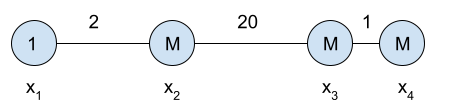
\includegraphics[width=0.6\textwidth]{Images/SingleLinkageC.png}
    \caption{Αντιπαράδειγμα του single-linkage}
    \label{fig:singleGR}
\end{figure}

Είναι εύκολο να δούμε ότι η βέλτιστη λύση είναι να τοποθετήσουμε τα κέντρα στις θέσεις $x_2$,$x_3$ και $x_4$ και να εξυπηρετήσουμε τον $x_1$ από το κέντρο στο $x_2$. Το συνολικό κόστος της βέλτιστης λύσης είναι 2. Όμως ο single-linkage θα ενώσει σε ένα cluster τις θέσεις $x_3$ και $x_4$. Αυτή η λύση όμως έχει κόστος $M$.

Με μία μικρή τροποποίηση στον παραπάνω αλγόριθμο μπορούμε να παίρνουμε πάντα τη βέλτιστη λύση σε ευσταθή στιγμιότυπα. Αντί να σταματάμε στα $k$ clusters συνεχίζουμε μέχρι να μείνει ένα cluster και στη συνέχεια με δυναμικό προγραμματισμό μπορούμε να βρούμε το βέλτιστο $k$-clustering.

\begin{lemmagr} 
O single-linkage αλγόριθμος βρίσκει πάντα τη βέλτιστη λύση αν, και μόνο αν, κάθε βέλτιστο cluster είναι υποδέντρο του ελάχιστου συνεκτικού δέντρου.
\end{lemmagr}

\begin{figure}[ht]
    \centering
    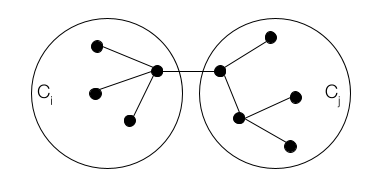
\includegraphics[width=0.5\textwidth]{Images/MSTconnected.png}
    \caption{Τα βέλτιστα cluster είναι υποδέντρα του ΕΣΔ.}
    \label{fig:MSTCon}
\end{figure}

Το παραπάνω λήμμα ισχύει διότι o single-linkage μπορεί να φτιάξει $k$-clusterings αφαιρώντας $k-1$ ακμές από το δέντρο. Αν τα clusters δεν είναι υποδέντρα δεν υπάρχει τρόπος να τα φτιάξει.

\begin{lemmagr}[\cite{Angelidakis2017}]
Ο single-linkage βρίσκει τη βέλτιστη λύση για κάθε 2-ευσταθές στιγμιότυπο.  
\end{lemmagr}


\section{Προβλήματα Χωροθέτησης σε Ευσταθή Στιγμιότυπα}

Όπως είδαμε και παραπάνω η βασική δυσκολία των προβλημάτων χωροθέτησης είναι:
\begin{enumerate}[(i)]
    \item Αν θέλουμε φραγμένο λόγο προσέγγισης πρέπει να τοποθετήσουμε τις υπηρεσίες βάση των αποστάσεων μεταξύ των παικτών. Έτσι όμως οι μηχανισμοί δεν είναι φιλαλήθης. 
    \item  Αν θέλουμε φιλαλήθης μηχανισμούς δεν πρέπει να ``κοιτάμε" το στιγμιότυπο. Έτσι όμως οι μηχανισμοί δεν έχουν φραγμένο λόγο προσέγγισης.
\end{enumerate}

Αν όμως υποθέσουμε ότι τα πραγματικά στιγμιότυπα είναι ευσταθή, μπορούμε να σχεδιάσουμε μηχανισμούς με καλύτερες εγγυήσεις; Τα βέλτιστα cluster στα ευσταθή στιγμιότυπα είναι εύκολα διαχωρίσιμα που σημαίνει ότι μπορούμε να τοποθετήσουμε μία υπηρεσία σε κάθε βέλτιστο cluster για να έχουμε φραγμένο λόγο προσέγγισης αλλά ταυτόχρονα οι παίκτες έχουν λιγότερη δύναμη στο να αλλάξουν τα βέλτιστα cluster. Αξίζει να σημειώσουμε ότι αυτό δεν είναι εφικτό χωρίς να υποθέσουμε ότι το στιγμιότυπο είναι ευσταθές, ακόμα και δύο υπηρεσίες στη γραμμή.

%Αν υποθέσουμε ότι το στιγμιότυπο είναι ευσταθές, μπορούμε να χρησιμοποιήσουμε τη δομή που έχει για να σχεδιάσουμε καλύτερους μηχανισμούς. 
Η βασική διαφορά μεταξύ της προηγούμενης ενότητας και αυτής είναι ότι οι παίκτες είναι στρατηγικοί. Κάθε παίκτης έχει το δικαίωμα να δηλώσει οποιαδήποτε θέση επιθυμεί ανεξάρτητα από τη πραγματική του. Αντίθετα, οι διαταραχές που χρησιμοποιούμε για να δείξουμε ότι ένα στιγμιότυπο είναι ευσταθές παράγονται με συγκεκριμένο τρόπο. Από εδώ και πέρα, θα υποθέσουμε ότι τα πραγματικά στιγμιότυπα που θα έχει να χειριστεί ένας μηχανισμός είναι ευσταθή και θα μελετήσουμε τη δύναμη που έχει ένας παίκτη να αλλάξει την έξοδο του μηχανισμού. 

%\begin{definitiongr}[$\g$-διαταραχή και $\g$-ευστάθεια]

%\end{definitiongr}
Για τα ευσταθή στιγμιότυπα έχουμε δύο πολύ σημαντικές ιδιότητες που θα μας φανούν πολύ χρήσιμες στη συνέχεια.

\begin{lemmagr}\label{con}
Έστω ένα $\g$-ευσταθές στιγμιότυπο $\x$, με $\g\ge2$. Τότε κάθε βέλτιστο cluster είναι υποδέντρο του δέντρου.
\end{lemmagr}

\begin{lemmagr}
Έστω ένα $\g$-ευσταθές στιγμιότυπο, με $\g\ge2+\sqrt{3}$. Από το cluster separation property έχουμε ότι για κάθε τοποθεσία $x_i$ κάθε εσωτερική απόσταση είναι μικρότερη από κάθε εξωτερική:
\[ d(x_i,x_j) \ge d(x_i,x_i') \; \forall x_i,x_i;\in C_i \;\&\; x_j \in C_j\]
\end{lemmagr}

Μια αρνητική παρατήρηση για τη βέλτιστη λύση είναι ότι δεν είναι φιλαλήθης αν περιέχει έστω και ένα cluster με ένα μόνο παίκτη (singleton cluster). Ας υποθέσουμε ότι το πραγματικό στιγμιότυπο είναι αυτή της εικόνας \ref{fig:original}. Αν ένας παίκτης δηλώσει μια θέση ``πολύ μακριά" από τους υπόλοιπους παίκτες τότε θα έχει μια υπηρεσία στη θέση που δήλωσε ενώ το υπόλοιπο στιγμιότυπο θα εξυπηρετηθεί από $k-1$ υπηρεσίες. Όπως φαίνεται και στη εικόνα \ref{fig:deviation} τα δύο cluster θα ενωθούν και έτσι ο παίκτης που δήλωσε ψευδή θέση κατάφερε να φέρει μια υπηρεσία πιο κοντά στη πραγματική του θέση. Το πρόβλημα είναι ότι και τα δύο στιγμιότυπα είναι $\g$-ευσταθή και δεν μπορούμε με κάποιο τρόπο να διαχωρίσουμε αν το στιγμιότυπο είναι πραγματικό ή αν έχει προκύψει από κάποια αλλαγή. Παρόλα αυτά, στα πραγματικά στιγμιότυπα που μοντελοποιούν προβλήματα χωροθέτησης υπηρεσιών είναι φυσικό να υποθέσουμε ότι δεν υπάρχουν singleton clusters. 



\begin{figure}[ht]
\centering
    \begin{subfigure}[b]{0.35\textwidth}
         \centering
         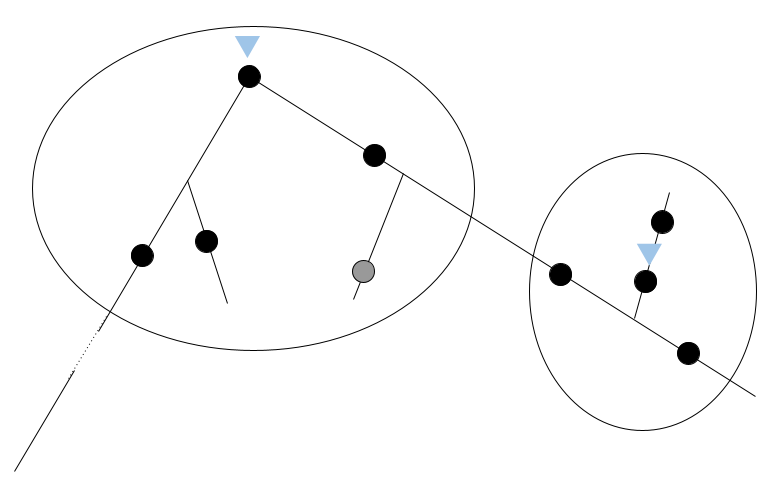
\includegraphics[width=\textwidth]{Images/stable1.png}
         \caption{Αρχικό στιγμιότυπο}
         \label{fig:original}
     \end{subfigure}
    \hspace{50pt}
    \begin{subfigure}[b]{0.35\textwidth}
         \centering
         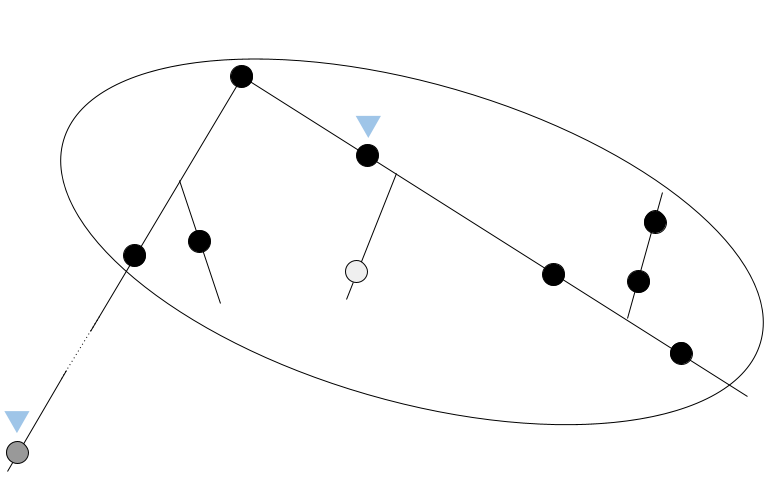
\includegraphics[width=\textwidth]{Images/stable2.png}
         \caption{Το στιγμιότυπο μετά την αλλαγή.}
         \label{fig:deviation}
     \end{subfigure}
    \end{figure}

\begin{algorithm}[ht]
\label{algorithm:optimalgr}
\DontPrintSemicolon
\SetAlgoLined
\LinesNumbered
\KwResult{Μια ανάθεση $k$-υπηρεσιών}
\KwIn{Ένα στιγμιότυπο $\x$ $k$-Facility Location.}
Υπολογισμός του βέλτιστου clustering
 $(C_1, \ldots, C_k)$. Έστω $c_i$ η διάμεση θέση του cluster $C_i$.\;

 \uIf{\big($\exists i \in [k]$ with $|C_i|=1$\big) or \big($\exists \;x_i,x_i'\in Ci$ and  $x_j,x_j'\in C_j$ with $\max\{ d(x_i,x_i'), d(x_j,x_j')\} \geq d(x_i,x_j) $\big)}{
 \KwOut {``Δεν τοποθετούνται υπηρεσίες''.}}\uElse{
 
\KwOut {Οι $k$-υπηρεσίες τοποθετούνται στις θέσεις $(c_1, \ldots, c_k)$ \;}}

\caption{\textsc{Optimal}}
\end{algorithm}

Το δεύτερο βήμα του αλγορίθμου λειτουργεί ως βήμα επαλήθευσης. Το cluster separation property είναι αναγκαία συνθήκη για την ευστάθεια, επομένως αν έχει παραβιαστεί είμαστε σίγουροι ότι κάποιος παίκτης έχει δηλώσει ψευδή τοποθεσία. Αν όμως ένα στιγμιότυπο ``περάσει" τον έλεγχο δεν σημαίνει ότι είναι ευσταθές. Επίσης, να σημειώσουμε ότι μπορούμε αποδοτικά να ελέγξουμε όλες τις απαραίτητες αποστάσεις. Σύμφωνα με το λήμμα \ref{con} κάθε βέλτιστο cluster είναι υποδέντρο του δέντρου, επομένως αρκεί να ελέγξουμε τις $k-1$ ακμές μεταξύ των διαφορετικών cluster.


\begin{theoremgr}
Ο \textsc{Optimal} μηχανισμός είναι φιλαλήθης και βέλτιστος για το πρόβλημα χωροθέτησης υπηρεσιών όταν το στιγμιότυπο είναι $2+\sqrt{3}$ ευσταθές.
\end{theoremgr}




\begin{proof}[Sketch]
Έστω ένας παίκτης που ανήκει στο $C_i$ δηλώνει μια άλλη τοποθεσία με σκοπό να φέρει μια υπηρεσία πιο κοντά στη πραγματική του τοποθεσία. Ο μόνος τρόπος που μπορεί να το πετύχει αυτό είναι να δηλώσει μια θέση $x_i'$ τέτοια ώστε στη περιοχή που πήγε να χρειαστεί μια επιπλέον υπηρεσία για να τους εξυπηρετήσει (το τοπικό κόστος αυξήθηκε). Αυτό έχει ως αποτέλεσμα το $C_i$ να ενωθεί με το γειτονικό του (το τοπικό κόστος μειώθηκε). Όπως φαίνεται και στην εικόνα από κάτω η υπηρεσία στο συνενωμένο cluster είναι πιο κοντά από την υπηρεσία που θα τον εξυπηρετούσε αν έλεγε την αλήθεια. 

Όμως επειδή το στιγμιότυπο είναι ευσταθές είτε τα δύο γειτονικά cluster στη περιοχή που πήγε ο $x_i$ θα παραβιάζουν την ελάχιστη εξωτερική απόσταση είτε αυτή η αλλαγή δεν θα είναι εφικτή. Μπορούμε να προσομοιώσουμε την αλλαγή στα κόστη με μια $\g$-διαταραχή. Αφού το αρχικό στιγμιότυπο είναι ευσταθές το βέλτιστο clustering δεν αλλάζει. Όμως, αυτό σημαίνει ότι ο μηχανισμός δεν θα έκανε αυτή την αλλαγή ούτε στο στιγμιότυπο που ο $x_i$ έχει δηλώσει τη θέση $x_i'$.


\begin{figure}[ht]
    \centering
    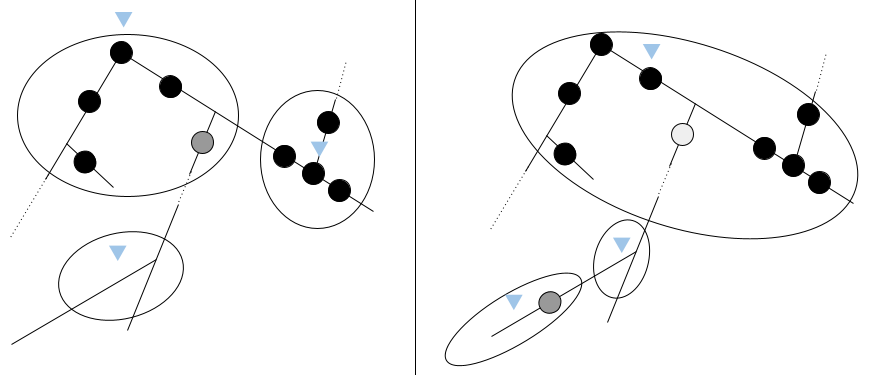
\includegraphics[width=0.7\textwidth]{Images/Deviation.png}
    \caption{Πιθανή κερδοφόρα αλλαγή}
    \label{fig:profDev}
\end{figure}
\end{proof}\


\section{Ανοιχτά προβλήματα}

Στις παραπάνω ενότητες είδαμε τα βασικά αποτελέσματα για το πρόβλημα χωροθέτησης υπηρεσιών αλλά και από που πηγάζει η δυσκολία του προβλήματος. Επιπλέον, είδαμε πως αν εστιάσουμε στα ``πραγματικά" στιγμιότυπα, από τη σκοπιά της ανάλυσης των αλγορίθμων πέρα της χειρότερης περίπτωσης, μπορούμε σχεδιάσουμε καλύτερους αλγορίθμους για προβλήματα που είναι πολύ δύσκολα στη γενική περίπτωση.Στον \textsc{Optimal} μηχανισμό είδαμε ότι πρέπει να αποκλείσουμε τα στιγμιότυπα που περιέχουν singleton clusters διότι ένας παίκτης μπορεί να δηλώσει μια θέση πολύ μακριά για να κερδίσει. Για να αντιμετωπίσουμε αυτό το πρόβλημα μια ενδιαφέρουσα ιδέα είναι να περιορίσουμε το εύρος των πιθανών τοποθεσιών που μπορεί να δηλώσει κάθε παίκτης σε σχέση με τη πραγματική του τοποθεσία. Σε αυτή τη περίπτωση πρέπει να δούμε πόσο ευσταθές πρέπει να είναι το στιγμιότυπο ώστε η βέλτιστη λύση να είναι φιλαλήθης. Μια άλλη κατεύθυνση είναι να ``χαλαρώσουμε" τον ορισμό της ευστάθειας σε ένα που είναι πιο πιθανό να περιγράφει τα πραγματικά στιγμιότυπα. Έχει προταθεί στη βιβλιογραφία για το clustering τα $(\g,\epsilon)$-ευσταθή στιγμιότυπα, στα οποία  για κάθε γ-διαταραχή το πολύ ένα μικρό ποσοστό $\epsilon$ σημείων αλλάζουν cluster.